
\documentclass[12pt]{report}

\usepackage[margin=1in,includefoot]{geometry}
\usepackage{graphicx}
\usepackage[hidelinks]{hyperref}
\usepackage{float}

\begin{document}

\begin{titlepage}
	\begin{center}
		\line(1,0){0}\\
		[4cm]
		\huge{\bfseries Pattern Recognition} \\
		[0.5cm]
		Assignment \#1 \\
		[0.5cm]
		\large{SVD-EVD and Regression} \\
		[10cm]
	\end{center}
	\begin{center}
		
			\Large{
			  Professor:  \hfill  Nirav Bhavsar (CS17S016)\\
		  Hema A. Murthy  \hfill  Sidharth Aggarwal (CS17S012)\\
			}
	
	
	\end{center}
	
\end{titlepage}

\tableofcontents
\thispagestyle{empty}
\cleardoublepage

\setcounter{page}{1}

%\setcounter{chapter}{1}

\chapter{Singular Value Decomposition}

We will perform Singular Value Decomposition on both square and rectangular images.

(a) by converting the image to grayscale.

(b) separately on each color bands.

(c) after concatenating the 8bit R,G,B channel to form a 24bit number. 

\section{SVD on Square Image by converting to Gray scale}

The singular value decomposition of any $ m\times n $  real or complex matrix $ \mathbf  M $  is a factorization of the form  $ \mathbf{ U\Sigma V^{*} }$ where $ \mathbf {U} $ and $ \mathbf {V} $ are real or complex unitary matrix, $ \mathbf{\Sigma} $ is a diagonal matrix with non-negative real numbers on the diagonal called Singular Values.\\

To compute SVD of a Matrix, we first find Eigen values $\mathbf{\Lambda}$ and Eigen vectors $\mathbf{X}$ of $ \mathbf{A'*A} $, then eigen vector $\mathbf{X}$ would be $\mathbf{V}$ and  $\mathbf{\Lambda}$ will be equal to $\mathbf{\Sigma^{2}}$. Then, to compute $\mathbf{U}$ we will calculate $\mathbf{A*V*\Sigma^{-1}}$ \\

Now, we will convert our original image to gray scale image and perform SVD and reconstruct original image using  $ \mathbf{ U\Sigma V^{*} }$.

\begin{figure}[H]
	\centering
	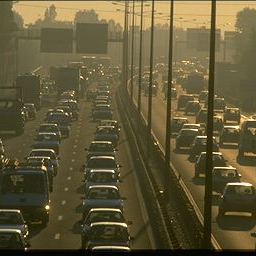
\includegraphics[scale=.5]{/Users/NiravMBA/Desktop/Report/18_Square.jpg}
	\caption{Original Square image}
\end{figure}

\begin{figure}[H]
	\centering	
	\includegraphics[scale=0.24]{/Users/NiravMBA/Desktop/Report/SVD_GraySquare1.jpg}
	\caption{Original Gray Scale \& Reconstructed Square image}
\end{figure}

Now, we will select Top N singular values of $ \mathbf{\Sigma} $ and reconstruct image along with it's corresponding error image with respect to original image.\\

\begin{figure}[H]

	\includegraphics[width=\linewidth]{/Users/NiravMBA/Desktop/Report/SVD_GraySquare.jpg}
	\caption{SVD on Gray Scale Square image}
\end{figure}


Below graph shows how Frobenius Norm of error image decreases as we select more top N singular values. \\
\begin{figure}[H]
	\centering
	\includegraphics[scale=0.5]{/Users/NiravMBA/Desktop/Report/SVD_GraySquare2.jpg}
	\caption{Graph of Frobenius Norm Vs Top N singular values of Gray scale square image}
\end{figure}

\cleardoublepage

\section{SVD on Square Image by seperating it's Red color band}

Similarly, we extract red color band from original image and perform SVD and select top N singular values and reconstruct original image along with it's corresponding error image.\\

\begin{figure}[H]
	
	\includegraphics[width=\linewidth]{/Users/NiravMBA/Desktop/Report/SVD_SquareRed1.jpg}
	\caption{SVD on Red color band of Square image}
\end{figure}

\cleardoublepage
\section{SVD on Square Image by seperating it's Green color band}

Similarly, we extract green color band from original image and perform SVD and select top N singular values and reconstruct original image along with it's corresponding error image.\\


\begin{figure}[H]
	
	\includegraphics[width=\linewidth]{/Users/NiravMBA/Desktop/Report/SVD_SquareGreen1.jpg}
	\caption{SVD on Green color band of Square image}
\end{figure}

\cleardoublepage

\section{SVD on Square Image by seperating it's Blue color band}

Similarly, we extract blue color band from original image and perform SVD and select top N singular values and reconstruct original image along with it's corresponding error image.\\


\begin{figure}[H]
	
	\includegraphics[width=\linewidth]{/Users/NiravMBA/Desktop/Report/SVD_SquareBlue1.jpg}
	\caption{SVD on Blue color band of Square image}
\end{figure}

\cleardoublepage

\section{SVD on Square Image after concatenating the 8bit R,G,B channel as RGB to form a 24bit number }

We extract 8bit R,G,B color bands from original image, then concatenate into a 24bit number as R then G then B and perform SVD and select top N singular values and reconstruct original image along with it's corresponding error image.\\

\begin{figure}[H]
	
	\includegraphics[width=\linewidth]{/Users/NiravMBA/Desktop/Report/SVD_SquareConcatRGB1.jpg}
	\caption{SVD on Square image concatenated at RGB}
\end{figure}
\cleardoublepage

\section{SVD on Square Image after concatenating the 8bit R,G,B channel as BRG to form a 24bit number }

We extract 8bit R,G,B color bands from original image, then concatenate into a 24bit number as B then R then G and perform SVD and select top N singular values and reconstruct original image along with it's corresponding error image.\\

\begin{figure}[H]
	
	\includegraphics[width=\linewidth]{/Users/NiravMBA/Desktop/Report/SVD_SquareConcatBRG1.jpg}
	\caption{SVD on Square image concatenated at BRG}
\end{figure}

\cleardoublepage

\section{SVD on Square Image after concatenating the 8bit R,G,B channel as GBR to form a 24bit number }

We extract 8bit R,G,B color bands from original image, then concatenate into a 24bit number as G then B then R and perform SVD and select top N singular values and reconstruct original image along with it's corresponding error image.\\

\begin{figure}[H]
	
	\includegraphics[width=\linewidth]{/Users/NiravMBA/Desktop/Report/SVD_SquareConcatGBR1.jpg}
	\caption{SVD on Square image concatenated at GBR}
\end{figure}

\cleardoublepage

\section{Comparitive Graph of reconstruction error vs N for 3 different methods of SVD on Square image }
 Below shows a comparison graph of reconstruction error vs N all three different methods namely \\  
 
 \begin{itemize}
 	\item Gray Scale
 	\item Three color bands - R,G,B
 	\item Three different types of concatenation of 8 bit R,G,B to 24 bit number
 \end{itemize}

\begin{figure}[H]
	
	\includegraphics[width=\linewidth]{/Users/NiravMBA/Desktop/Report/SVD_SquareGraph.jpg}
	\caption{Comparitive Graph of 3 methods of SVD}
\end{figure}

{\bfseries Observation: }
We observe that as we increase selecting top N singular values the Forbenius Norm Error of error image decreases and it follows almost similar curve for other
methods also after N = 30 singular value.  Also we observed from the images with permuted R,G,B bands that the color band 
in the last dominates the whole image. As you can see in RGB blue color is dominating, in 
GBR red is dominating and in BRG green color is dominating the whole image.\\

\cleardoublepage
%Rectangle Image SVD

\section{SVD on Rectangle Image by converting to Gray scale}
Similarly, we will perform same experiments for Rectangle image.

\begin{figure}[H]
	\centering
	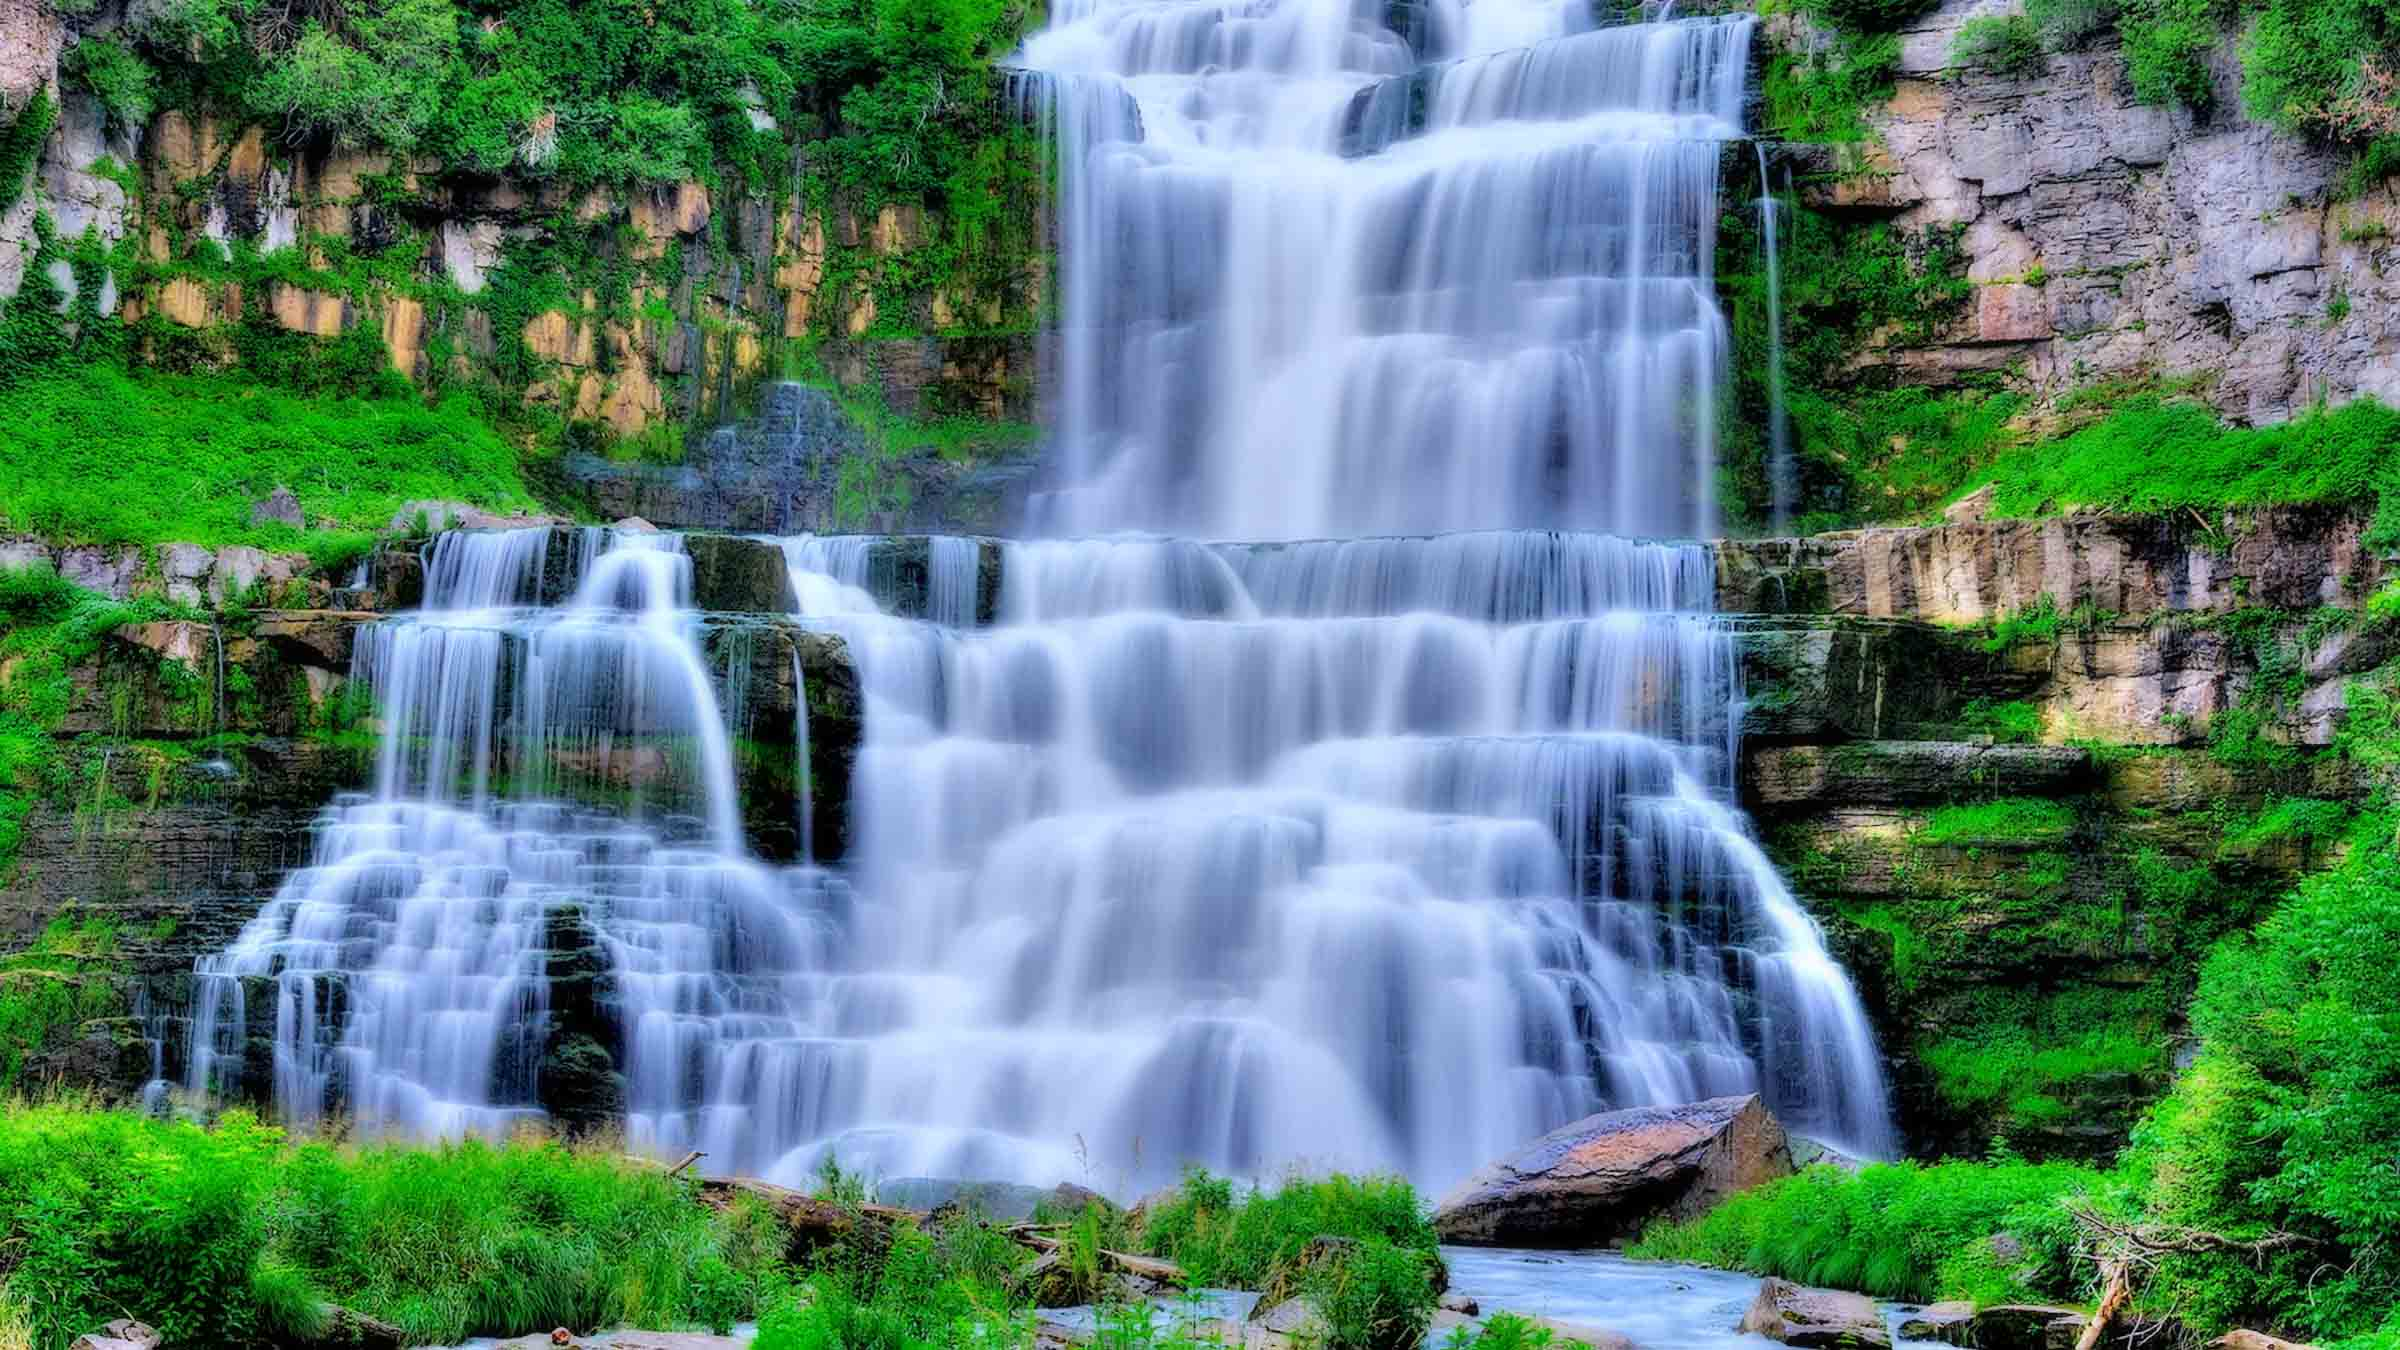
\includegraphics[scale=.45]{/Users/NiravMBA/Desktop/Report/18_Rect.jpg}
	\caption{Original Rectangle image}
\end{figure}


\begin{figure}[H]
	
	\includegraphics[width=\linewidth]{/Users/NiravMBA/Desktop/Report/SVD_RectGray1.jpg}
	\caption{SVD on Gray Scale Rectangle image}
\end{figure}

Below is the comparison graph of Frobenius Norm Vs Top N singular values of Gray scale Rectangle image. \\

\begin{figure}[H]
	
	\includegraphics[width=\linewidth]{/Users/NiravMBA/Desktop/Report/SVD_RectGray.jpg}
	\caption{Graph of Frobenius Norm Vs Top N singular values of Gray scale Rectangle image}
\end{figure}
\cleardoublepage

\section{SVD on Rectangle Image by seperating it's Red color band}

Similarly, we extract red color band from original image and perform SVD and select top N singular values and reconstruct original image along with it's corresponding error image.\\


\begin{figure}[H]
	
	\includegraphics[width=\linewidth]{/Users/NiravMBA/Desktop/Report/SVD_RectRed.jpg}
	\caption{SVD on Red color band of Rectangle image}
\end{figure}
\cleardoublepage

\section{SVD on Rectangle Image by seperating it's Green color band}

Similarly, we extract green color band from original image and perform SVD and select top N singular values and reconstruct original image along with it's corresponding error image.\\


\begin{figure}[H]
	
	\includegraphics[width=\linewidth]{/Users/NiravMBA/Desktop/Report/SVD_RectGreen.jpg}
	\caption{SVD on Green color band of Rectangle image}
\end{figure}
\cleardoublepage

\section{SVD on Rectangle Image by seperating it's Blue color band}

Similarly, we extract blue color band from original image and perform SVD and select top N singular values and reconstruct original image along with it's corresponding error image.\\


\begin{figure}[H]
	
	\includegraphics[width=\linewidth]{/Users/NiravMBA/Desktop/Report/SVD_RectBlue.jpg}
	\caption{SVD on Blue color band of Rectangle image}
\end{figure}

\cleardoublepage

\section{SVD on Rectangle Image after concatenating the 8bit R,G,B channel as RGB to form a 24bit number }

We extract 8bit R,G,B color bands from original image, then concatenate into a 24bit number as R then G then B and perform SVD and select top N singular values and reconstruct original image along with it's corresponding error image.\\

\begin{figure}[H]
	
	\includegraphics[width=\linewidth]{/Users/NiravMBA/Desktop/Report/SVD_RectRGB.jpg}
	\caption{SVD on Rectangle image concatenated at RGB}
\end{figure}
\cleardoublepage

\section{SVD on Rectangle Image after concatenating the 8bit R,G,B channel as BRG to form a 24bit number }

We extract 8bit R,G,B color bands from original image, then concatenate into a 24bit number as B then R then G and perform SVD and select top N singular values and reconstruct original image along with it's corresponding error image.\\

\begin{figure}[H]
	
	\includegraphics[width=\linewidth]{/Users/NiravMBA/Desktop/Report/SVD_RectBRG.jpg}
	\caption{SVD on Rectangle image concatenated at BRG}
\end{figure}
\cleardoublepage

\section{SVD on Rectangle Image after concatenating the 8bit R,G,B channel as GBR to form a 24bit number }

We extract 8bit R,G,B color bands from original image, then concatenate into a 24bit number as G then B then R and perform SVD and select top N singular values and reconstruct original image along with it's corresponding error image.\\

\begin{figure}[H]
	
	\includegraphics[width=\linewidth]{/Users/NiravMBA/Desktop/Report/SVD_RectGBR.jpg}
	\caption{SVD on Rectangle image concatenated at GBR}
\end{figure}
\cleardoublepage

\section{Comparitive Graph of reconstruction error vs N for 3 different methods of SVD on Rectangle image }

Below shows a comparison graph of reconstruction error vs N all three different methods namely \\  

\begin{itemize}
	\item Gray Scale
	\item Three color bands - R,G,B
	\item Three different types of concatenation of 8 bit R,G,B to 24 bit number
\end{itemize}


\begin{figure}[H]
	
	\includegraphics[width=\linewidth]{/Users/NiravMBA/Desktop/Report/SVD_RectGraph1.jpg}
	\caption{Comparitive Graph of 3 methods of SVD}
\end{figure}

{\bfseries Observation: }
We observe that as we increase selecting top N singular values the Forbenius Norm Error of error image decreases and it follows almost similar curve for other
methods also. Also we observed from the images with permuted R,G,B bands that the color band 
in the center dominates the whole image. As you can see in RGB green color is dominating, in 
GBR blue is dominating and in BRG red color is dominating the whole image.\\


% Eigen Values


\chapter{Eigen Value Decomposition}

We will perform Eigen Value Decomposition on both square and rectangular images.

(a) by converting the image to grayscale.

(b) separately on each color bands.

(c) after concatenating the 8bit R,G,B channel to form a 24bit number. 

\section{EVD on Square Image by converting to Gray scale}

Eigen Value Decomposition is the factorization of a matrix in terms of its eigenvalues and eigenvectors.
A Matric $ A $ can be factorized as
$ \mathbf{A}=\mathbf{Q}\mathbf{\Lambda}\mathbf{Q}^{-1}  $ 
where $ Q $ is the square $\mathbf{N\times N} $ matrix whose ith column is the eigenvector $ q_{i} $ of $ A $ and $ \Lambda $ is the diagonal matrix whose diagonal elements are the corresponding eigenvalues.\\

First we will convert original image to gray scale and then perform Eigen Value Decomposition and reconstruct original image using $ \mathbf{A}=\mathbf{Q}\mathbf{\Lambda}\mathbf{Q}^{-1}  $ 

\begin{figure}[H]
	\centering
	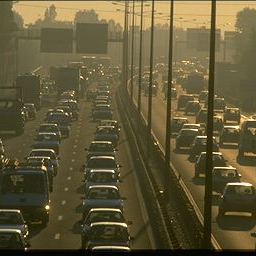
\includegraphics[scale=.5]{/Users/NiravMBA/Desktop/Report/18_Square.jpg}
	\caption{Original Square image}
\end{figure}

\begin{figure}[H]
	\centering	
	\includegraphics[scale=0.3]{/Users/NiravMBA/Desktop/Report/EVD_Square_Gray.jpg}
	\caption{Original Gray Scale \& Reconstructed Square image}
\end{figure}

Now, we will select Top N eigen values of $ \mathbf{\Lambda} $ and reconstruct image along with it's corresponding error image with respect to original image.\\

\begin{figure}[H]
	
	\includegraphics[width=\linewidth]{/Users/NiravMBA/Desktop/Report/EVD_SQUARE_GRAY_2.jpg}
	\caption{EVD on Gray Scale Square image}
\end{figure}

Below graph shows how Frobenius Norm of error image decreases as we select more top N eigen values. \\

\begin{figure}[H]
	
	\includegraphics[width=\linewidth]{/Users/NiravMBA/Desktop/Report/EVD_SquareGrayGraph.jpg}
	\caption{Graph of Frobenius Norm Vs Top N eigen values of Gray scale square image}
\end{figure}
\cleardoublepage

\section{EVD on Square Image by seperating it's Red color band}

Similarly, we extract red color band from original image and perform EVD and select top N eigen values and reconstruct original image along with it's corresponding error image.\\

\begin{figure}[H]
	
	\includegraphics[width=\linewidth]{/Users/NiravMBA/Desktop/Report/EVD_SQUARE_RED.jpg}
	\caption{EVD on Red color band of Square image}
\end{figure}
\cleardoublepage
\section{EVD on Square Image by seperating it's Green color band}
Similarly, we extract green color band from original image and perform EVD and select top N eigen values and reconstruct original image along with it's corresponding error image.\\

\begin{figure}[H]
	
	\includegraphics[width=\linewidth]{/Users/NiravMBA/Desktop/Report/EVD_SQUARE_GREEN.jpg}
	\caption{EVD on Green color band of Square image}
\end{figure}
\cleardoublepage
\section{EVD on Square Image by seperating it's Blue color band}
Similarly, we extract blue color band from original image and perform EVD and select top N eigen values and reconstruct original image along with it's corresponding error image.\\

\begin{figure}[H]
	
	\includegraphics[width=\linewidth]{/Users/NiravMBA/Desktop/Report/EVD_SQUARE_BLUE.jpg}
	\caption{EVD on Blue color band of Square image}
\end{figure}
\cleardoublepage


\section{EVD on Square Image after concatenating the 8bit R,G,B channel as RGB to form a 24bit number }

We extract 8bit R,G,B color bands from original image, then concatenate into a 24bit number as R then G then B and perform EVD and select top N eigen values and reconstruct original image along with it's corresponding error image.\\

\begin{figure}[H]
	
	\includegraphics[width=\linewidth]{/Users/NiravMBA/Desktop/Report/EVD_SQUARE_CONCAT_RGB.jpg}
	\caption{EVD on Square image concatenated at RGB}
\end{figure}
\cleardoublepage
\section{EVD on Square Image after concatenating the 8bit R,G,B channel as BRG to form a 24bit number }
We extract 8bit R,G,B color bands from original image, then concatenate into a 24bit number as B then R then G and perform EVD and select top N eigen values and reconstruct original image along with it's corresponding error image.\\

\begin{figure}[H]
	
	\includegraphics[width=\linewidth]{/Users/NiravMBA/Desktop/Report/EVD_SQUARE_CONCAT_BRG.jpg}
	\caption{EVD on Square image concatenated at BRG}
\end{figure}

\cleardoublepage
\section{EVD on Square Image after concatenating the 8bit R,G,B channel as GBR to form a 24bit number }

We extract 8bit R,G,B color bands from original image, then concatenate into a 24bit number as G then B then R and perform EVD and select top N eigen values and reconstruct original image along with it's corresponding error image.\\

\begin{figure}[H]
	
	\includegraphics[width=\linewidth]{/Users/NiravMBA/Desktop/Report/EVD_SQUARE_CONCAT_GBR.jpg}
	\caption{EVD on Square image concatenated at GBR}
\end{figure}
\cleardoublepage

\section{Comparitive Graph of reconstruction error vs N for 3 different methods of EVD on Square image }
Below shows a comparison graph of reconstruction error vs N all three different methods namely \\  

\begin{itemize}
	\item Gray Scale
	\item Three color bands - R,G,B
	\item Three different types of concatenation of 8 bit R,G,B to 24 bit number
\end{itemize}


\begin{figure}[H]
	
	\includegraphics[width=\linewidth]{/Users/NiravMBA/Desktop/Report/EVD_Square_Graph.jpg}
	\caption{Comparitive Graph of 3 methods of EVD}
\end{figure}


{\bfseries Observation: }
We observe that as we increase selecting top N eigen values the Forbenius Norm Error of error image decreases. And error is more when red component is more in proportion to other in image for eigen values upto 150 while for other method they stabilises and decreases gradually after eigen value 30.\\

\cleardoublepage



\section{Comparitive Graph of reconstruction error vs N for 3 different methods of EVD \& SVD on Square image }

Below shows a comparison graph between SVD \& EVD of reconstruction error vs N for all three different methods namely \\  

\begin{itemize}
	\item Gray Scale
	\item Three color bands - R,G,B
	\item Three different types of concatenation of 8 bit R,G,B to 24 bit number
\end{itemize}

\begin{figure}[H]
	
	\includegraphics[width=\linewidth]{/Users/NiravMBA/Desktop/Report/EVD_SVD_SquareCompareGraph.jpg}
	\caption{Comparitive Graph of 3 methods of EVD \& SVD}
\end{figure}


{\bfseries Observation: }
We observe that as we increase selecting top N eigen/singular values the Forbenius Norm Error of error image decreases. For SVD the graph is smooth and it keeps on gradually decreasing with increase in N, While graph of EVD is not smooth it spikes up when red component is more in image. SVD error decreases rapildy to 2000 at N = 35 while EVD takes N = 180 to reach at 2000 error. \\

\cleardoublepage

%
%%Rectangle Image EVD

\section{EVD on Rectangle Image by converting to Gray scale}

%We will perform same experiments for Rectangle image.
To perform Eigen Value Decomposition for rectangle image $ \mathbf{A} $, we first find eigen values $ \mathbf{\Lambda} $ and eigen vector $ \mathbf{Q} $ for matrix $ \mathbf{A*A'} $, then we use formula $ \mathbf{M}=\mathbf{Q}\mathbf{\Lambda}\mathbf{Q}^{-1}  $  to reconstrust $ \mathbf{A*A'} $. We then multiply reconstructed matrix $ \mathbf{M} $ with pseudo inverse of $ \mathbf{A'} $ which is $ \mathbf{ (A*A')^{-1}*A } $ to reconstrust original image $ \mathbf{A} $.

\begin{figure}[H]
	\centering
	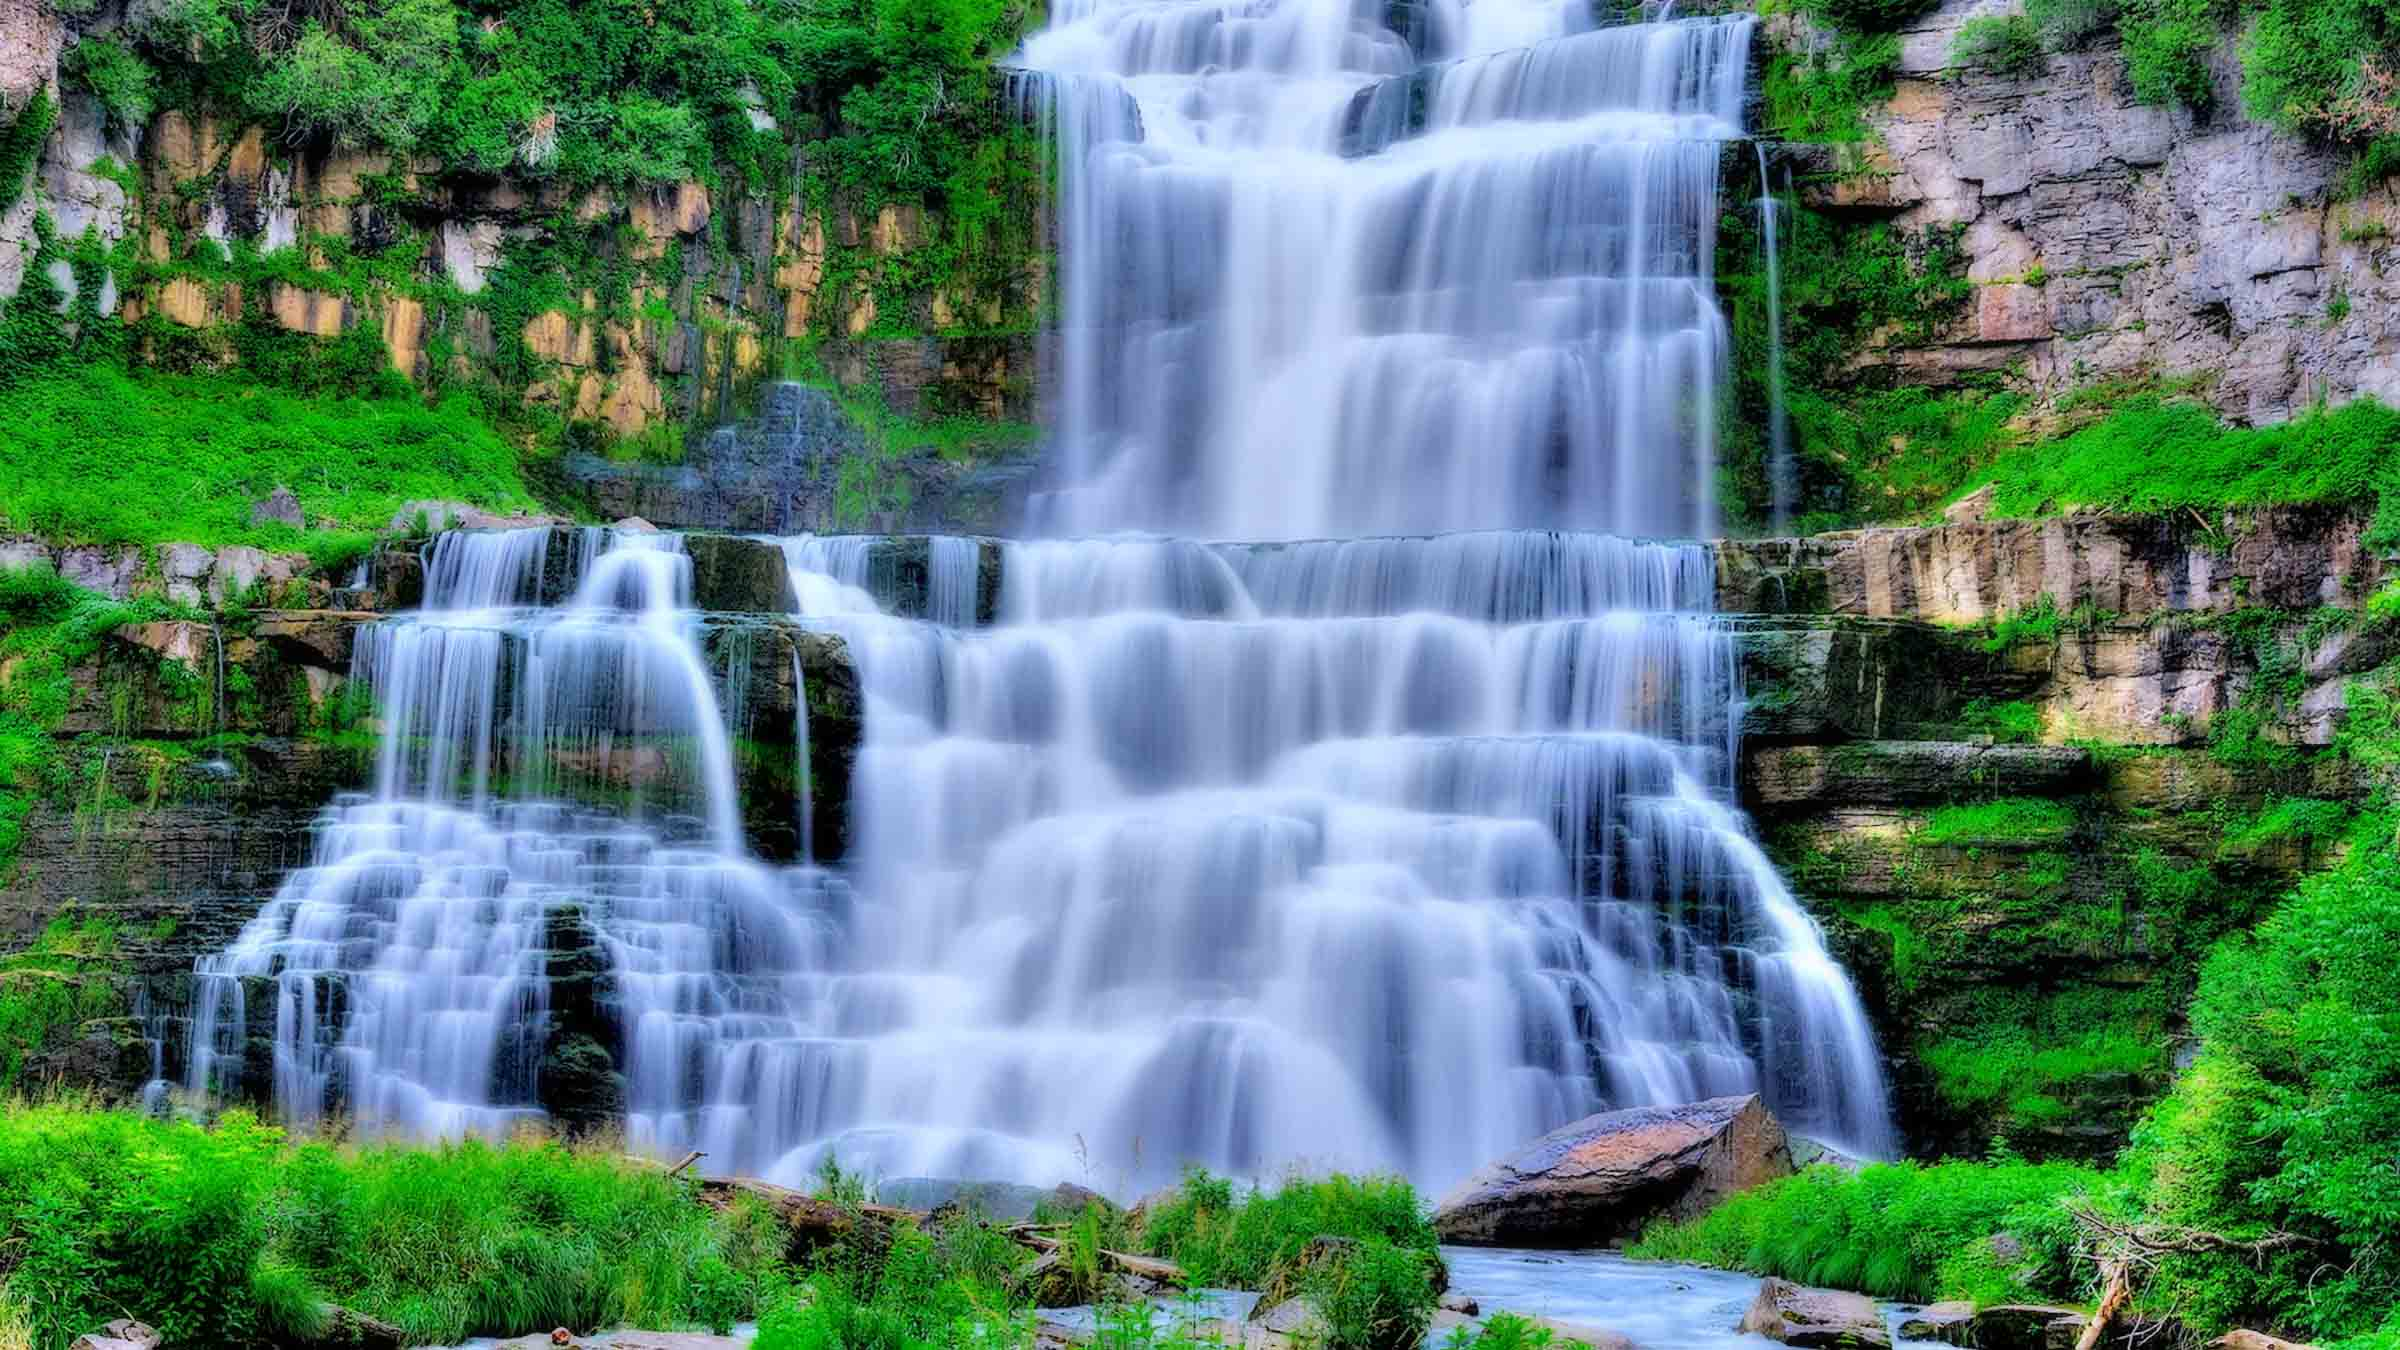
\includegraphics[scale=.5]{/Users/NiravMBA/Desktop/Report/18_Rect.jpg}
	\caption{Original Rectangle image}
\end{figure}


\begin{figure}[H]
	
	\includegraphics[width=\linewidth]{/Users/NiravMBA/Desktop/Report/EVD_REC_ORI_GRAY.jpg}
	\caption{Original Gray Scale \& Reconstructed Rectangle image using EVD}
\end{figure}
\cleardoublepage


Now, we will select Top N eigen values of $ \mathbf{\Lambda} $ and reconstruct image along with it's corresponding error image with respect to original image.\\

\begin{figure}[H]
	
	\includegraphics[width=\linewidth]{/Users/NiravMBA/Desktop/Report/EVD_REC_GRAY.jpg}
	\caption{EVD on Gray Scale Rectangle image}
\end{figure}
\cleardoublepage
%
%Below is the comparison graph of Frobenius Norm Vs Top N eigen values of Gray scale Rectangle image. \\
%\begin{figure}[H]
%	
%	\includegraphics[width=\linewidth]{/Users/NiravMBA/Desktop/Report/EVD_RectGray.jpg}
%	\caption{Graph of Frobenius Norm Vs Top N eigen values of Gray scale Rectangle image}
%\end{figure}
%\cleardoublepage

\section{EVD on Rectangle Image by seperating it's Red color band}

Similarly, we extract red color band from original image and perform EVD and select top N eigen values and reconstruct original image along with it's corresponding error image.\\


\begin{figure}[H]
	
	\includegraphics[width=\linewidth]{/Users/NiravMBA/Desktop/Report/EVD_REC_RED.jpg}
	\caption{EVD on Red color band of Rectangle image}
\end{figure}
\cleardoublepage
\section{EVD on Rectangle Image by seperating it's Green color band}
Similarly, we extract green color band from original image and perform EVD and select top N eigen values and reconstruct original image along with it's corresponding error image.\\


\begin{figure}[H]
	
	\includegraphics[width=\linewidth]{/Users/NiravMBA/Desktop/Report/EVD_REC_GREEN.jpg}
	\caption{EVD on Green color band of Rectangle image}
\end{figure}
\cleardoublepage

\section{EVD on Rectangle Image by seperating it's Blue color band}
Similarly, we extract blue color band from original image and perform EVD and select top N eigen values and reconstruct original image along with it's corresponding error image.\\


\begin{figure}[H]
	
	\includegraphics[width=\linewidth]{/Users/NiravMBA/Desktop/Report/EVD_REC_BLUE.jpg}
	\caption{EVD on Blue color band of Rectangle image}
\end{figure}

\cleardoublepage

\section{EVD on Rectangle Image after concatenating the 8bit R,G,B channel as RGB to form a 24bit number }

We extract 8bit R,G,B color bands from original image, then concatenate into a 24bit number as R then G then B and perform EVD and select top N eigen values and reconstruct original image along with it's corresponding error image.\\



\begin{figure}[H]
	
	\includegraphics[width=\linewidth]{/Users/NiravMBA/Desktop/Report/EVD_REC_CONCAT_RGB.jpg}
	\caption{EVD on Rectangle image concatenated at RGB}
\end{figure}
\cleardoublepage
\section{EVD on Rectangle Image after concatenating the 8bit R,G,B channel as BRG to form a 24bit number }

We extract 8bit R,G,B color bands from original image, then concatenate into a 24bit number as B then R then G and perform EVD and select top N eigen values and reconstruct original image along with it's corresponding error image.\\



\begin{figure}[H]
	
	\includegraphics[width=\linewidth]{/Users/NiravMBA/Desktop/Report/EVD_REC_CONCAT_BRG.jpg}
	\caption{EVD on Rectangle image concatenated at BRG}
\end{figure}
\cleardoublepage

\section{EVD on Rectangle Image after concatenating the 8bit R,G,B channel as GBR to form a 24bit number }

We extract 8bit R,G,B color bands from original image, then concatenate into a 24bit number as G then B then R and perform EVD and select top N eigen values and reconstruct original image along with it's corresponding error image.\\


\begin{figure}[H]
	
	\includegraphics[width=\linewidth]{/Users/NiravMBA/Desktop/Report/EVD_REC_CONCAT_GBR.jpg}
	\caption{EVD on Rectangle image concatenated at GBR}
\end{figure}
\cleardoublepage

\section{Comparitive Graph of reconstruction error vs N for 3 different methods of EVD on Rectangle image }

Below shows a comparison graph of reconstruction error vs N all three different methods namely \\  

\begin{itemize}
	\item Gray Scale
	\item Three color bands - R,G,B
	\item Three different types of concatenation of 8 bit R,G,B to 24 bit number
\end{itemize}


\begin{figure}[H]
	
	\includegraphics[width=\linewidth]{/Users/NiravMBA/Desktop/Report/EVD_REC_COMP_N.jpg}
	\caption{Comparitive Graph of 3 methods of EVD}
\end{figure}


{\bfseries Observation: }
We observe that as we increase selecting top N eigen values the Forbenius Norm Error of error image decreases and it follows almost similar curve for other methods also.\\

\cleardoublepage

\section{Comparitive Graph of reconstruction error vs N for 3 different methods of EVD \& SVD on Rectangle image }

Below shows a comparison graph between SVD \& EVD of reconstruction error vs N for all three different methods namely \\  

\begin{itemize}
	\item Gray Scale
	\item Three color bands - R,G,B
	\item Three different types of concatenation of 8 bit R,G,B to 24 bit number
\end{itemize}

\begin{figure}[H]
	
	\includegraphics[width=\linewidth]{/Users/NiravMBA/Desktop/Report/REC_EVD_SVD_Graph.jpg}
	\caption{Comparitive Graph of 3 methods of EVD \& SVD}
\end{figure}


{\bfseries Observation: }
We observe that as we increase selecting top N eigen/singular values the Forbenius Norm Error of error image decreases. For both EVD \& SVD the graph is almost similar and it keeps on gradually decreasing with increase in N. \\

\cleardoublepage


\chapter{Polynomial Regression}

The goal of regression analysis is to model the expected value of a dependent variable y in terms of the value of an independent variable (or vector of independent variables) x. In general, we can model the expected value of y as an nth degree polynomial, yielding the general polynomial regression model.

\begin{center}
	$ {\displaystyle y=\beta _{0}+\beta _{1}x+\beta _{2}x^{2}+\beta _{3}x^{3}+\cdots +\beta _{n}x^{n}+\varepsilon .\,} $\\
\end{center}

To come up with the best model which fits the give data we will try out with different orders of polynomial of input features x. Then for every model with polynomial order $ M $ we will find out mininum parameter which will give is it's best line/curve for that model by using normal equation.

\begin{center}
	$ {\displaystyle { {\theta }=(\mathbf {X} ^{\mathbf {T}}\mathbf {X} )^{-1} \mathbf {X} ^{\mathbf {T}} {y}}} $
\end{center}

By using this parameter $ {\theta } $ we will test our model on validation data and calculate Sum of Squared Error, then whichever models gives minimum value of error will be selected as best model for given data.\\

We will divide out data set into three parts:

\begin{itemize}
	\item Training data - 70%
	\item Validation data - 20%
	\item Testing data - 10%
\end{itemize}

We will find parameter $ {\theta } $ for every model from training data and then we will use that parameter $ {\theta } $ to calculate estimated value for validation data using $ \mathbf{E} = {X}*{\theta } $ and find Sum of Squared Error between estimated and actual output. Then select one which gives minimum error.\\


\section{1-dimensional data}


Below figure shows SSE Vs Degree for testing and validation data, we can see as we increase degree the error for training data decreases but error for validation data increases which means we are overfitting our parameters on input data so it will not work correctly for new unseen data, hence error increases for validation data.\\

\begin{figure}[H]
	
	\includegraphics[width=\linewidth]{/Users/NiravMBA/Desktop/Report/1DSSEVsDegree.jpg}
	\caption{SSE Vs Degree for 1D training and validation data}
\end{figure}

Now from above graph observation, we will select degree M as 5 since it is giving minium error for validation data. Then we will use parameter $ {\theta } $ for degree 5 which we calculated from training data on testing data to estimate output.\\

\begin{figure}[H]
	\centering
	\includegraphics[scale=0.26]{/Users/NiravMBA/Desktop/Report/1DTestingData.jpg}
	\caption{Plotting polynomial for M = 5 on testing data}
\end{figure}

And below is graph of Actual output Vs Estimated output for selected parameter $ {\theta } $ and degree M = 5.

\begin{figure}[H]
	
	\includegraphics[scale=0.28]{/Users/NiravMBA/Desktop/Report/1DTestingTar.jpg}
	\caption{Actual output Vs Estimated output}
\end{figure}


{\bfseries Observation: } 
We observe how error decreases as we increase degree for training data but error for validation data increases which means we are overfitting our parameters on input data so it will not work correctly for new unseen data, hence error increases for validation data.


\section{Ridge Regression on 1-dimensional data}

As we saw in previous experiment our error increases with increase in degree for unseen validation data, means it the regression model becomes tailored to fit the quirks and random noise in your specific sample rather than to approximate the true model.\\
 So, as we increase the degree of M the value of coefficiencts in parameter $ \mathbf{\theta} $ increases to very high value, so to control this we add regularization parameter $ \mathbf{\Lambda} $ to our original formula for finding parameter $ \mathbf{\theta} $.

\begin{center}
	$ {\displaystyle { {\theta }=(\mathbf {X} ^{\mathbf {T}}\mathbf {X} + \mathbf{\Lambda} )^{-1} \mathbf {X} ^{\mathbf {T}} {y}}} $
\end{center}

We will try out different models with different order of polynomial degree and different  $ \mathbf{\Lambda} $ to find out which gives least error on validation data.

\begin{figure}[H]
	\centering
	\includegraphics[scale=0.35]{/Users/NiravMBA/Desktop/Report/1De-2.jpg}
	\caption{1D Training Data with polynomial of degree 4 and lambda e\^-2} 
\end{figure}

\begin{figure}[H]
	\centering
	\includegraphics[scale=0.35]{/Users/NiravMBA/Desktop/Report/1De-8.jpg}
	\caption{1D Training Data with polynomial of degree 6 and lambda e\^-8} 
\end{figure}


%\cleardoublepage

Now, we will try out with different values of $ \mathbf{\lambda} $ on few models to find which lambda is best for our data. Below is graph of SSE Vs Lambda for M = 5 \& 15.

\begin{figure}[H]
	\centering
	\includegraphics[scale=0.23]{/Users/NiravMBA/Desktop/Report/1Dlamdam5.jpg}
	\caption{SSE Vs Lambda for M = 5 on  training and validation data} 
\end{figure}


\begin{figure}[H]
	\centering
	\includegraphics[scale=0.3]{/Users/NiravMBA/Desktop/Report/1Dlambdam15.jpg}
	\caption{SSE Vs Lambda for M = 15 on  training and validation data} 
\end{figure}

We observe that as value of $ \mathbf{\lambda} $ increases, error increases as we are making coefficeints of parameter $ \mathbf{\theta} $ small and eventually it stabilizes and follows straight line. For higher order polynomial also the error is same and regulariation works with few fluctuations. And we can observe that validation error is less compared to training error as we have not allowed data to overfit on training data. Thus we select lambda = e\^-8 as it error is low and it stabilies around that. \\

Below figure shows SSE Vs Degree for testing and validation data, we can observe  how error decreases as we increasing the degree and since we have used regulariation the error is high for training data but less for validation data as we have reduced coefficients of higher order through regulariation. \\

\begin{figure}[H]
	\centering
	\includegraphics[scale=0.26]{/Users/NiravMBA/Desktop/Report/1DSSEe-8.jpg}
	\caption{SSE Vs Degree for 1D ridge training and validation data for lambda = e\^-8  \& M = 8} 
\end{figure}




Now from above graph observation, we will select degree lambda = e\^-8  and M as 8 since it is stable around that order for validation data. Then we will use parameter $ {\theta } $ for degree 5 which we calculated from training data on testing data to estimate output.\\

\begin{figure}[H]
	\centering
	\includegraphics[scale=0.26]{/Users/NiravMBA/Desktop/Report/1DTesting.jpg}
	\caption{Plotting polynomial for M = 8 and lambda = e\^-8 on testing data} 
\end{figure}

\cleardoublepage
And below is graph of Actual output Vs Estimated output for selected parameter $ {\theta } $ and degree M = 8 and lambda = e\^-8.

\begin{figure}[H]
	
	\includegraphics[scale=0.3]{/Users/NiravMBA/Desktop/Report/1DTargetridge.jpg}
	\caption{Actual output Vs Estimated output} 
\end{figure}


{\bfseries Observation: } 
We observe how error decreases slowly as we increase degree for training data and as we are using lambda = e\^-8 it's error is more compared to validation dara as we are not allowing data to overfit and error decreases for validation data so it will work correctly for new unseen data.

\section{2-dimensional data}

Now we will perform polymonial regression on 2-dimensional data. We will try out different models with different order of polynomial degree and find out which gives least error on validation data.\\

Below is the plot of training data with polynomial of degree 1,2 \& 3\\
\begin{figure}[H]
	\centering
	\includegraphics[scale=0.25]{/Users/NiravMBA/Desktop/Report/2Dtrainm1.jpg}
		\includegraphics[scale=0.25]{/Users/NiravMBA/Desktop/Report/2Dtraimm2.jpg}
			\includegraphics[scale=0.25]{/Users/NiravMBA/Desktop/Report/2Dtraimm3.jpg}
	\caption{2D Training Data with polynomial of degree 1,2 \& 3 }
\end{figure}


Below figure shows SSE Vs Degree for testing and validation data, we can observe  how error decreases as we increasing the degree and it stabilies to zero after degree 7.\\ 

\begin{figure}[H]
	\centering
	\includegraphics[scale=0.3]{/Users/NiravMBA/Desktop/Report/2DSSEVsDeg.jpg}
	\caption{SSE Vs Degree for 2D training and validation data }
\end{figure}



Now from above graph observation, we will select degree M as 7 since it is giving minium error for validation data. Then we will use parameter $ {\theta } $ for degree 7 which we calculated from training data on testing data to estimate output.\\

\begin{figure}[H]
	
	\includegraphics[scale=0.32]{/Users/NiravMBA/Desktop/Report/2D_TESTING.jpg}
	\caption{Plotting polynomial for M = 7 on testing data}
\end{figure}

And below is graph of Actual output Vs Estimated output for selected parameter $ {\theta } $ and degree M = 5.


\begin{figure}[H]
	
	\includegraphics[scale=0.32]{/Users/NiravMBA/Desktop/Report/2D_TARGET.jpg}
	\caption{Actual output Vs Estimated output}
\end{figure}

{\bfseries Observation: } 
We observe how error decreases as we increase degree for training data, but since error becomes almost close to zero which means we have accurately predicted best model for our data, hence error becomes zero for unseen validation data also.



\cleardoublepage

\section{Ridge Regression on 2-dimensional data}


Now we will perform ridge regression, We will try out different models with different order of polynomial degree and different  $ \mathbf{\Lambda} $ to find out which gives least error on validation data.

\begin{figure}[H]
	\centering
	\includegraphics[scale=0.3]{/Users/NiravMBA/Desktop/Report/2D_RIDGE_M2_TRAINING.jpg}
	\caption{Multi Dimension Training Data with polynomial of degree 2 and lambda e\^-5} 
\end{figure}

\begin{figure}[H]
	\centering
	\includegraphics[scale=0.3]{/Users/NiravMBA/Desktop/Report/2D_RIDGE_M3_TRAINING.jpg}
	\caption{Multi Dimension Training Data with polynomial of degree 3 and lambda e\^-4} 
\end{figure}

\begin{figure}[H]
	\centering
	\includegraphics[scale=0.3]{/Users/NiravMBA/Desktop/Report/2D_RIDGE_M5_TRAINING.jpg}
	\caption{Multi Dimension Training Data with polynomial of degree 5 and lambda e\^-3} 
\end{figure}

Now, we will try out with different values of $ \mathbf{\lambda} $ on few models to find which lambda is best for our data. Below is graph of SSE Vs Lambda for M = 5 \& 7.\\

\begin{figure}[H]
	\centering
	\includegraphics[scale=0.3]{/Users/NiravMBA/Desktop/Report/2D_SSE_RIDGE_M5.jpg}
	\caption{SSE Vs Lambda for M = 5 on training and validation data} 
\end{figure}


\begin{figure}[H]
	\centering
	\includegraphics[scale=0.3]{/Users/NiravMBA/Desktop/Report/2D_SSE_RIDGE_M7.jpg}
	\caption{SSE Vs Lambda for M = 7 on training and validation data} 
\end{figure}

We observe that as value of $ \mathbf{\lambda} $ increases, error increases as we are making coefficeints of parameter $ \mathbf{\theta} $ small and eventually it stabilizes and follows straight line. For higher order polynomial also the error is same and regulariation works with few fluctuations. Thus we select lambda = e\^-8 as error is low and it stabilies around that. \\

Below figure shows SSE Vs Degree for testing and validation data, we can observe error is low for lower order of polynomial and error increasing then stabilises for higher degree. \\

\begin{figure}[H]
	\centering
	\includegraphics[scale=0.32]{/Users/NiravMBA/Desktop/Report/2D_SSE_VS_DEGREE_RIDGE_E6.jpg}
	\caption{SSE Vs Degree for Multi dimension ridge training and validation data for lambda = e\^-6  \& M = 7} 
\end{figure}


Now from above graph observation, we will select degree lambda = e\^-8  and M as 7 since it is stable around that order for validation data. Then we will use parameter $ {\theta } $ for degree 7 which we calculated from training data on testing data to estimate output.\\

\begin{figure}[H]
	\centering
	\includegraphics[scale=0.3]{/Users/NiravMBA/Desktop/Report/2D_TESTING.jpg}
	\caption{Plotting polynomial for M = 7 and lambda = e\^-6 on testing data} 
\end{figure}


And below is graph of Actual output Vs Estimated output for selected parameter $ {\theta } $ and degree M = 7 and lambda = e\^-8.

\begin{figure}[H]
	
	\includegraphics[scale=0.35]{/Users/NiravMBA/Desktop/Report/2D_TARGET5.jpg}
	\caption{Actual output Vs Estimated output} 
\end{figure}


{\bfseries Observation: } 
We observe how error decreases as we increase degree for lambda = e\^-6 training data, but since error becomes almost close to zero which means we have accurately predicted best model for our data, hence error becomes zero for unseen validation data also.

\section{Multidimensional data}

Similarly, we will perform same experiment for Multi-dimensional data. First we will calculate parameter $ \mathbf{\theta} $ for different order of polynomial from training data and use those parameter on validation data to find out best model i.e order of polynomial which gives least error.\\ \\ 
Before performing experiment we observed data and found that two columns of data are same, which will not add any more information to our model hence we didn't consider that column for calculating parameter $ \mathbf{\theta} $\\

\begin{figure}[H]
	\centering
	\includegraphics[scale=0.23]{/Users/NiravMBA/Desktop/Report/MDSSEVsDegree.jpg}
	\caption{SSE Vs Degree for Multi-Dimension on training and validation data} 
\end{figure}

From the above graph we observe that it gives least error for M = 7. Hence we will select M as 7 as use our calculated parameter $ \mathbf{\theta} $ from training data on test data and plot Actual output Vs Estimated output graph which show how good/bad our model works on unseen test data.\\

\begin{figure}[H]
	\centering
	\includegraphics[scale=0.23]{/Users/NiravMBA/Desktop/Report/MDTarget.jpg}
	\caption{Actual output Vs Estimated output} 
\end{figure}

{\bfseries Observation: } 
We observe how error decreases as we increase degree for training data but error increases for few higher order then it again decreases and we observe similar curve for validation data also but with far less error, which means our prediction is close to accurate.

\section{Ridge Regression on Multidimensional data}

Now we will perform ridge regression, We will try out different models with different order of polynomial degree and different  $ \mathbf{\Lambda} $ to find out which gives least error on validation data.


\begin{figure}[H]
	\centering
	\includegraphics[scale=0.24]{/Users/NiravMBA/Desktop/Report/3dridgem6.jpg}
	\caption{SSE Vs Lambda for M = 6 on training and validation data} 
\end{figure}


\begin{figure}[H]
	\centering
	\includegraphics[scale=0.24]{/Users/NiravMBA/Desktop/Report/3dridgem7.jpg}
	\caption{SSE Vs Lambda for M = 7 on training and validation data} 
\end{figure}

We observe that as value of $ \mathbf{\lambda} $ increases, error increases as we are making coefficeints of parameter $ \mathbf{\theta} $ small and eventually it stabilizes and follows straight line. For higher order polynomial also the error is same and regulariation works with few fluctuations. And we can observe that validation error is less compared to training error as we have not allowed data to overfit on training data. Thus we select lambda = e\^-8 as it error is low and it stabilies around that. \\

Below figure shows SSE Vs Degree for testing and validation data, we can observe error is low for lower order of polynomial and error increasing then stabilises for higher degree and since we have used regulariation the error is high for training data but less for validation data as we have reduced coefficients of higher order through regulariation. \\

\begin{figure}[H]
	\centering
	\includegraphics[scale=0.23]{/Users/NiravMBA/Desktop/Report/3dridgesse10.jpg}
	\caption{SSE Vs Degree for 1D ridge training and validation data for lambda = e\^-8  \& M = 7} 
\end{figure}


Now from above graph observation, we will select degree lambda = e\^-10  and M as 7 since it is stable around that order for validation data. Then we will use parameter $ {\theta } $ for degree 5 which we calculated from training data on testing data to estimate output and plot graph of Actual output Vs Estimated output.\\


\begin{figure}[H]
	
	\includegraphics[scale=0.3]{/Users/NiravMBA/Desktop/Report/3dridgetarget.jpg}
	\caption{Actual output Vs Estimated output} 
\end{figure}

{\bfseries Observation: } 
We observe how error decreases as we increase degree for training data but error does increases for few higher order as we have use regularisation with lambda = e\^-8 which limits coefficients to take large value and we observe similar curve for validation data also but with far less error, which means our prediction is close to accurate.

\end{document}
			